\documentclass[11pt,a4paper]{report}

\usepackage{url}
\usepackage{graphicx}
\title{Installation of an Operating System on Raspberry Pi }
\author{e-Yantra summer internship 2017}
\date{\today}

\begin{document}
	\maketitle
	\newpage
	\tableofcontents
	\newpage
	\section{Objective}
	This tutorial will help a Windows or a Linux user to install an operating system on Raspberry Pi successfully.
	\section{Prerequisites}
	\begin{itemize}
		\item An idea about Windows or Linux operating system and their features.
	\end{itemize}
	\section{Hardware Requirement}
	\begin{enumerate}
		\item Raspberry Pi (I will be using Version 2 Model-B)
		\item Adapter (To power up an R-pi)
		\item SD card reader
		\item PC (either Linux or Windows machine)
	\end{enumerate}
	\section{Software Requirement}
	\begin{enumerate}
		\item Winrar or any other zipping software 
		\item Utorrent or any suitable downloading platform	
		\item win32DiskManager
	\end{enumerate}
	\newpage
	\section{Theory and Description}
	The Raspberry Pi is a series of small single-board computers developed in the United Kingdom by the Raspberry Pi Foundation.Raspberry Pi is a low cost, credit-card sized computer that plugs into a computer monitor or TV, and uses a standard keyboard and mouse. It is a capable little device that enables people of all ages to explore computing, and to learn how to program in languages like Scratch and Python.The Raspberry Pi 2 uses a Broadcom BCM2836 SoC with a 900 MHz 32-bit quad-core ARM Cortex-A7 processor, with 256 KB shared L2 cache It’s capable of doing everything you’d expect a desktop computer to do, from browsing the internet and playing high-definition video, to making spreadsheets, word-processing, and playing games.
	
	\subsection{A comparison between different models and versions of Raspberry pi}
\resizebox{\textwidth}{!}{	\begin{tabular}{ | p{1in} | p{1in} | p{1in} | p{1in } | p{1in} | p{1in} |}	
	\hline
	Parameter & Model A & Model A+ & Model B & Model B+ & Generation 2 Model B \\
   	\hline	
	\textbf{Target price(in US dollars):} & 25 & 20 & 35 & 25 & 35 \\
	\hline	
	\textbf{SoC:} & Broadcom BCM2835 (CPU, GPU, DSP, SDRAM, one USB port) & Broadcom BCM2835 (CPU, GPU, DSP, SDRAM, one USB port) & Broadcom BCM2835 (CPU, GPU, DSP, SDRAM, one USB port) & Broadcom BCM2835 (CPU, GPU, DSP, SDRAM, one USB port) & Broadcom BCM2836 (CPU, GPU, DSP, SDRAM, one USB port) \\
	\hline 
	\textbf{CPU:} & 700 MHz single-core ARM1176JZF-S & 700 MHz single-core ARM1176JZF-S & 700 MHz single-core ARM1176JZF-S & 700 MHz single-core ARM1176JZF-S & 900 MHz quad-core ARM Cortex-A7 \\
	\hline	
	\textbf{Memory (SDRAM):} & 256 MB (shared with GPU)	512 MB & 256 MB (shared with GPU) & 512 MB (shared with GPU) & 512 MB (shared with GPU) & 1 GB (shared with GPU) \\
	\hline 
	\textbf{USB 2.0 ports:} & 1 (direct from BCM2835 chip) & 1 (direct from BCM2835 chip) & 2 (via the on-board 3-port USB hub)[38] & 4 (via the on-board 5-port USB hub) & 4 (via the on-board 5-port USB hub) \\
	\hline 
	\textbf{On-board storage:} & SD / MMC / SDIO card slot (3.3 V with card power only) & MicroSD slot[32] & SD / MMC / SDIO card slot & MicroSD slot & MicroSD slot \\
	\hline
	\textbf{On-board network:} & None & None & 10/100 Mbit/s Ethernet (8P8C) USB adapter on the third/fifth port of the USB hub (SMSC lan9514-jzx) & 10/100 Mbit/s Ethernet (8P8C) USB adapter on the third/fifth port of the USB hub (SMSC lan9514-jzx) & 10/100 Mbit/s Ethernet (8P8C) USB adapter on the third/fifth port of the USB hub (SMSC lan9514-jzx) \\
	\hline 
	\textbf{Low-level peripherals:} & 8× GPIO & 17× GPIO plus the same specific functions, and HAT ID bus & 8× GPIO  & 17× GPIO  & 17× GPIO \\
	\hline
	\textbf{Power ratings:} & 300 mA (1.5 W) & 200 mA (1 W) &	700 mA (3.5 W) & 600 mA (3.0 W) & 800 mA(4.0 W) \\
	\hline 
	\end{tabular}}
	\centering
	Ref: [2]
	
	\newpage
	\flushleft
	\section{Experiment}
	Instructions for installing operating system in Raspberry Pi:
	
	Download Raspbian software from raspberry pi website. It should be available in the form of a zip file. Download it from the following link: \url{https://www.raspberrypi.org/downloads/} Also download win32DiskManager from the following link:\url{http://sourceforge.net/projects/win32diskimager/} and then install it.
	
	\vspace{0.5cm}
	A windows user should follow these steps:
	\begin{itemize}
		\item Insert an sd card(4GB or greater size) into the laptop in the memory card slot if available or use a memory card reader. Run win32DiskImager and choose the Raspbian image and select the drive corresponding to your sd card.
		\item Click "Write" to copy the files of the image on to the sd card.
		\item Eject SD card and insert it into the sd card slot of the Raspberry Pi.
	\end{itemize}
	
	A Linux user should follow these steps:
		\begin{itemize}
			\item Insert an sd card(4GB or greater size) into the laptop in the memory card slot if available or use a memory card reader.
			\item Run df -h to see what devices are currently mounted. The new device that has appeared is your SD card. The left column gives the device name of your SD card; it will be listed as something like /dev/mmcblk0p1 or /dev/sdd1. The last part (p1 or 1 respectively) is the partition number but you want to write to the whole SD card, not just one partition. Therefore you need to remove that part from the name (getting, for example, /dev/mmcblk0 or /dev/sdd) as the device for the whole SD card. Note that the SD card can show up more than once in the output of df; it will do this if you have previously written a Raspberry Pi image to this SD card, because the Raspberry Pi SD images have more than one partition.
			\item Note down your device name. You need to unmount it so that files can't be read or written to the SD card while you are copying over the SD image.
			\item Run umount /dev/sdd1, replacing sdd1 with whatever your SD card's device name is (including the partition number).
			If your SD card shows up more than once in the output of df due to having multiple partitions on the SD card, you should unmount all of these partitions.
			\item In the terminal, write the image to the card with the command below, making sure you replace the input file if= argument with the path to your .img file, and the /dev/sdd in the output file of= argument with the right device name. This is very important, as you will lose all data on the hard drive if you provide the wrong device name. Make sure the device name is the name of the whole SD card as described above, not just a partition of it; for example sdd, not sdds1 or sddp1; or mmcblk0, not mmcblk0p1.
			
			dd bs=4M if=2015-05-05-raspbian-wheezy.img of=/dev/sdd
			
			Please note that block size set to 4M will work most of the time; if not, please try 1M, although this will take considerably longer.
			
			Also note that if you are not logged in as root you will need to prefix this with sudo.
			\item The dd command does not give any information of its progress and so may appear to have frozen; it could take more than five minutes to finish writing to the card. If your card reader has an LED it may blink during the write process. To see the progress of the copy operation you can run pkill -USR1 -n -x dd in another terminal, prefixed with sudo if you are not logged in as root. The progress will be displayed in the original window and not the window with the pkill command; it may not display immediately, due to buffering.
			
			Instead of dd you can use dcfldd; it will give a progress report about how much has been written.
			
			You can check what's written to the SD card by dd-ing from the card back to another image on your hard disk, truncating the new image to the same size as the original, and then running diff (or md5sum) on those two images.
			
			\item The SD card might be bigger than the original image, and dd will make a copy of the whole card. We must therefore truncate the new image to the size of the original image. Make sure you replace the input file if= argument with the right device name. diff should report that the files are identical.
			
			dd bs=4M if=/dev/sdd of=from-sd-card.img
			truncate --reference 2015-05-05-raspbian-wheezy.img from-sd-card.img
			diff -s from-sd-card.img 2015-05-05-raspbian-wheezy.img
			\item Run sync; this will ensure the write cache is flushed and that it is safe to unmount your SD card.
			\item Remove the SD card from the card reader and insert it into Raspberry Pi's SD card slot. [1]
		\end{itemize}
		
	After inserting the SD card into Raspberry Pi follow these steps:
	\begin{enumerate}
		\item Connect the keyboard and mouse.Use HDMI cable to connect the board to the VGA monitor
		\item Power on the board and the monitor. You will notice a set of code running on the monitor.
		\item After a while a software configuration tool opens.
			\begin{figure}[h!]
				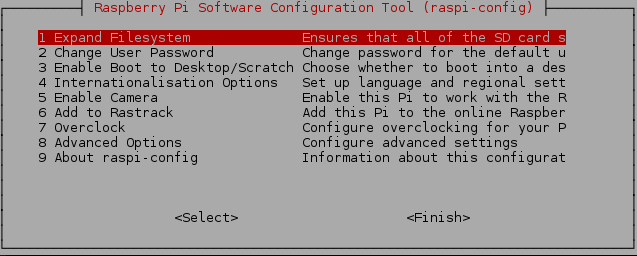
\includegraphics[scale=0.6]{2.PNG}
				\centering
			\end{figure}
		\item In case the size of the SD card is greater than 4GB you can select the 1st option i.e.Expand file system in the configuration tool as shown above.	
		\item Select the internationalisation options.
			\begin{figure}[h!]
				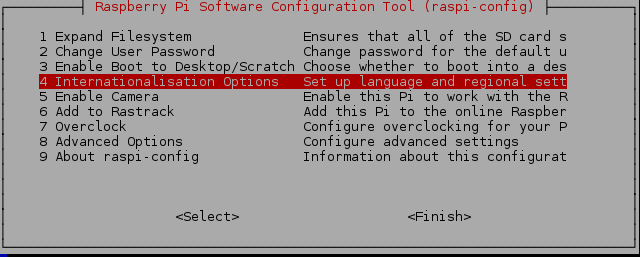
\includegraphics[scale=0.6]{3.PNG}
				\centering
			\end{figure}
		\item Change the keyboard and language settings as per your choice. Default keyboard will be of UK. Step by step change to US keyboard is as shown:
		\begin{itemize}
		\item First select the option change Keyboard layout and click ok
			\begin{figure}[h!]
				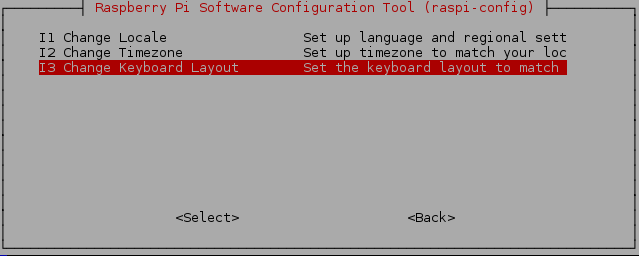
\includegraphics[scale=0.6]{4.PNG}
				\centering
			\end{figure}
		\newpage
		\item Then select the respective keyboard you are using and if you dont find your kind then select any of the generic types.
			\begin{figure}[h!]
				\includegraphics[width=10cm,height=10cm]{Keyboard-Change2.PNG}
				\centering
			\end{figure}
		\item Select "English US" which will be available at the top. Then for the rest of the process simply click enter till you reach the main configuration menu.
			\begin{figure}[h!]
				\includegraphics[scale=0.6]{Keyboard-Change3.PNG}
				\centering	
			\end{figure}
		\end{itemize}
	\newpage
	\item Click on finish using the keyboard by using arrow keys and enter key.
	\item Click on "ok" when prompted for reboot.
	\item Upon reboot, enter 'pi' as user id and 'raspberry' as password. Then type 'startx' to enter the graphical interface.
	\item The linux based raspbian interface will be displayed on the monitor. Some of the softwares will be preloaded such as wolfram, python etc.
	\item The command prompt will be the lx terminal.
	\end{enumerate}
	\flushleft
	With this we end the installation of Raspbian OS in R-Pi.
	\vspace{0.4cm} 
	\newpage
	\section{References}
	\begin{enumerate}
		\item \url{https://www.raspberrypi.org/}
		\item \url{http://en.wikipedia.org/wiki/Raspberry_Pi}	
		\item \url{https://www.raspberrypi.org/wp-content/uploads/2014/11/Raspberry_Pi_Family_A-annotated-15001.jpg}
		\item \url{http://assets.windowsphone.com/3f82dfe6-a179-4ddf-9738-91989190c3fa/IoT-rpi2-board_InvariantCulture_Default.png}	
	\end{enumerate}

\end{document}



